% -*- root: ../InvestigacionOperativa.tex -*-


\section{Conjuntos convexos}

Vamos a ver qué es un conjunto convexo como caso particular de conjuntos afines.
Dados 2 puntos $x_1,x_2$, y $\theta$, tomamos
\[
y = \theta x_1 + (1-\theta)x_2 = x_2 + \theta (x_1-x_2),\ \ \  x_1,x_2\in\mathbb{R}^n.
\]

Vamos a pensar qué ocurre diferentes valores de $\theta$:


\begin{figure}[h]
\begin{center}
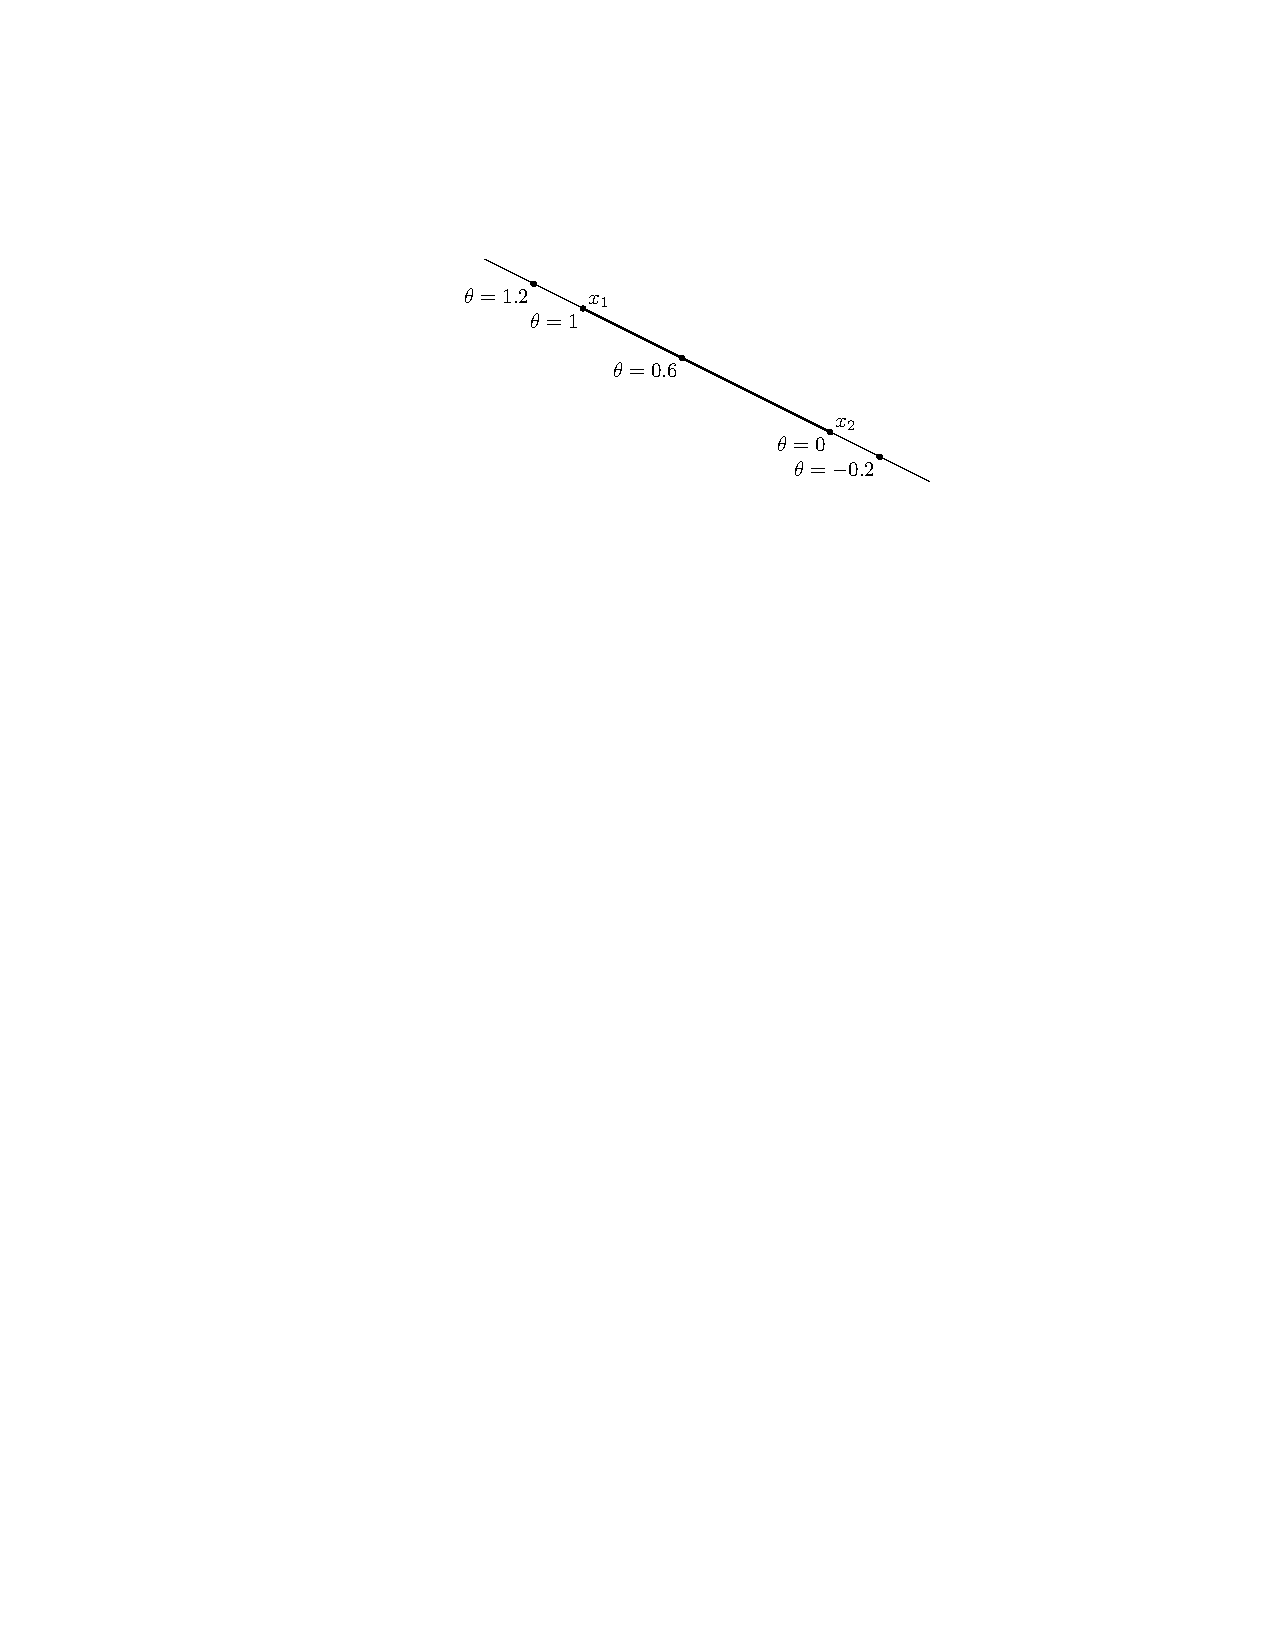
\includegraphics[scale=0.8]{pdf/berrendero/tema2/_combinacion}
\caption{Ejemplo de combinaciones lineales de 2 puntos para ilustrar conjuntos afin y convexo.}
\label{sec2:comb}
\end{center}
\end{figure}


En la figura $\ref{sec2:comb}$, vemos que podemos obtener distintos puntos de la recta dependiendo de $\theta$. La recta entera sería un conjunto afín (se obtiene con $\theta \in \real$), mientras que el segmento ($\theta \in [0,1]$) sería el conjunto convexo. Formalmente,

\begin{defn}[Conjunto\IS afín]
Dados $x_1,x_2\in S$, S es un conjunto afín si $\theta x_1 + (1-\theta)x_2\in S$, para todo $\theta\in \mathbb{R}$.
\end{defn}

\begin{defn}[Conjunto\IS convexo]
Dados $x_1,x_2\in S$, S es un conjunto convexo si $\theta x_1 + (1-\theta)x_2\in S$, para todo $\theta\in [0,1]$.
\end{defn}



Vamos a ver ejemplos de subconjuntos convexos. Conviene parar un momento a pensar cada uno de los ejemplos hasta convencerse de que son convexos.
\begin{itemize}
\item \textbf{Hiperplanos}: $S=\{x:\, p^\top x = \alpha\}$, donde $p\in\mathbb{R}^n$, $\alpha\in\mathbb{R}$.

\item \textbf{Semiespacios}: $S=\{x:\, p^\top x \leq \alpha\}$, donde $p\in\mathbb{R}^n$, $\alpha\in\mathbb{R}$.

\item \textbf{Intersección arbitraria} de convexos: Si $S_i$ es convexo para todo $i\in I$, entonces $S=\bigcap_{i=1}^I S_i$ es un conjunto convexo.

\item Un \textbf{poliedro} (intersección finita de semiespacios) es un conjunto convexo. Por ejemplo, $S=\{x:\, Ax\leq b,\ x\geq 0\}$ es un conjunto convexo.

\item Una \textbf{bola} $B(\bar x,r)=\{x\in\mathbb{R}^n:\, \|x-\bar x\|<r\}$ es un conjunto convexo (para cualquier norma).

\end{itemize}



\subsection{Combinaciones convexas y afines}

Hemos visto lo que son los conjuntos convexos, pero a la hora de trabajar, puede que el conjunto de datos con el que trabajamos, no sea convexo. ¿Tiene sentido hablar del "mínimo conjunto convexo" que contiene al conjunto con el que estamos trabajando?  Claro que sí, de hecho vamos a intentar construirlo. Para ello necesitamos definir qué es una combinación.

\begin{defn}[Combinación\IS afín]

Sean $x_1,\ldots,x_k \in\mathbb{R}^n$. Una combinación afín de $\{x_i\}$ es
\[
y = \lambda_1 x_1+\cdots +\lambda_k x_k,
\]
donde $\lambda_1+\cdots +\lambda_k=1$.
\end{defn}


En el caso de combinaciones convexas, tenemos alguna restricción más, ya que los conjuntos convexos son subconjuntos de conjuntos afines.

\begin{defn}[Combinación\IS convexa]
Sean $x_1,\ldots,x_k \in\mathbb{R}^n$. Una combinación convexa de $\{x_i\}$ es
\[
y = \lambda_1 x_1+\cdots +\lambda_k x_k,
\]
donde $\lambda_1+\cdots +\lambda_k=1$ y $\lambda_i \geq 0$, para todo $i=1,\ldots,n$.
\end{defn}


Ya tenemos los ingredientes para construir los \textbf{cierres}, es decir, los mínimos conjuntos convexos/afines que contienen a un conjunto.


\begin{defn}[Cierre\IS afín]
Definimos $\afin{S}$, el cierre afín de un conjunto $S$ como
\[
\afin{S} = \left\{\sum_{i=1}^k \lambda_i x_i:\, x_i\in S,\  \sum_{i=1}^k \lambda_i = 1\right\}.
\]
\end{defn}

\paragraph{Propiedades:}
\begin{itemize}
\item Un conjunto es afín si y solo $S=\afin{S}$.

\item Un conjunto es afín si y solo si es la traslación de un subespacio vectorial (único)

\item La dimensión afín de un conjunto es la dimensión de su cierre afín (que a su vez es la dimensión del correspondiente subespacio vectorial).
\end{itemize}




\begin{defn}[Cierre convexo]
Definimos $\convx{S}$, el cierre convexo de un conjunto $S$ como
\[
\convx{S} = \left\{\sum_{i=1}^k \lambda_i x_i:\, x_i\in S,\ \lambda_i\geq 0,\ \sum_{i=1}^k \lambda_i = 1\right\}.
\]
\end{defn}

\paragraph{Propiedades:}
\begin{itemize}
\item  S es convexo si y sólo si $S = \convx{S}$

\begin{proof} Vamos a separar las implicaciones:


$\impliedby)$:\\ $S = \convx{S} \implies S$ convexo es trivial, vamos a demostrar la otra implicación:

$\implies)$:\\ Queremos demostrar que si $S$ es convexo, $S\subset \convx{S}$ y $\convx{S}\subset S$. Es trivial que $S\subset\convx{S}$, asique vamos a ver la otra inclusión y vamos a demostrarlo por inducción sobre $k$. Sea

\[x = \sum_i^k λ_ix_i \text{ con } x_i \in S,λ\geq 0, \sum^k λ = 1\]

\subparagraph{Base:} $k=1$ es trivial.

\subparagraph{Paso:}Suponemos cierto para $k$ y tenemos que demostrarlo para $k+1$: \[\text{Hay que demostrar que si }\, x=\sum_{i=1}^{k+1} \lambda_i x_i \,, \text{ con }\,\sum_{i=1}^{k+1} \lambda_i = 1 \text{ y }\lambda_i \geq 0 \implies x \in S\]

Supongamos, sin pérdida de generalidad que $λ_{k+1} < 1$ y tomamos:
\[\sum^{k+1} λ_ix_i = (1-λ_{k+1})\underbrace{\left(\frac{λ_1}{1-λ_{k+1}}x_1 + ... + \frac{λ_k}{1-λ_{k+1}}x_k \right)}_{(1)}+λ_{k+1}x_{k+1}\]
$(1)$ es una combinación convexa (ya que $\sum_{i=1}^{k}\lambda_k = 1 - \lambda_{k+1}$), por tanto $(1)\in S$.

Por otro lado, $(1-λ_{k+1})a + λ_{k+1}x_{k+1}$ es una combinación convexa, ya que $a,x_{k+1}\in S$ y ambos coeficientes cumplen las restricciones.

Con ello, vemos que $\convx{S}\subset S$.
\end{proof}


\item $\convx{S}$ es el menor conjunto convexo que contiene a $S$

\end{itemize}


\begin{theorem}[Teorema\IS de Carathéodory]
Sea $S\subset \mathbb{R}^n$. Si $x\in\convx{S}$, entonces $x$ se puede escribir como combinación lineal de, como máximo, $n+1$ puntos de $S$.


Entonces \[x=\sum_{i=1}^{n+1}\lambda_i x_i\text{ con }\sum_{i=1}^{n+1}\lambda_i=1, \lambda_i\geq 0, x_i\in S,\; \forall i=1,\ldots, n+1\].
\end{theorem}

La demostración es interesante porque tiene un razonamiento que utilizaremos a menudo. Este razonamiento es: \textit{Perturbar un conjunto de coeficientes para que alguno llegue a ser 0, pero sin llegar a obtener ningún coeficiente negativo.
}

\begin{proof}
Sea $x\in\convx{S}$.

Vamos a tomar una combinación convexa con $k$ elementos. Entonces \[x=\sum_{i=1}^{k}\lambda_i x_i,\text{ con } \sum_{i=1}^{k}\lambda_i=1, \lambda_i> 0, x_i\in S\]



Si $k\leq n+1$, hemos terminado, ya que tenemos expresado $x$ como combinación convexa de, a lo más, $n+1$ componentes.

Ahora vamos a ver que si $k > n+1$, entonces podemos expresarlo como combinación convexa de $k-1$ elementos.

Por ser $k>n+1$, tenemos que $x_2-x_1,\ldots, x_k-x_1$ son linealmente dependientes (porque estamos en $\real^n$), entonces existen $\mu_i$ (alguno estrictamente positivo) tales que $\displaystyle\sum_{i=1}^{k}\mu_i x_i=0$.

Entonces, podemos escribir $x=\sum_{i=1}^k (\lambda_i-\alpha\mu_i)x_i$, donde
\[
\alpha = \min\{\lambda_j/\mu_j:\, \mu_j>0\}:=\lambda_r/\mu_r > 0.
\]

Este $\alpha$ lo obtenemos para mantener que sea una combinación convexa. Necesitaremos $λ_i - \alpha μ_i \geq 0$ y $\sum (λ_i -\alpha μ_i) = 1$

Tomando este $\alpha$ conseguimos expresar $x$ como combinación convexa de $k-1$ elementos. Si todavía $k>n+1$, volvemos al paso 1. En un número finito de iteraciones habremos llegado a $k = n+1$, con lo que habremos terminado la demostración.
\end{proof}



Sea $S\subset\mathbb{R}^n$ un convexo cuyo cierre afín es $\mbox{afin}(S)$. El \textbf{interior relativo} de $S$ se define como el conjunto de puntos $x\in S$ tales que existe $r>0$ con $B(x,r)\cap \mbox{afin}(S) \subset S$.

\begin{itemize}
\item ¿Cuál es el interior relativo de $\{x\in \mathbb{R}^3:\, -1\leq x_1\leq 1,\, -1\leq x_2\leq 1,\, x_3=0\}$?
\end{itemize}



\begin{theorem}
Un conjunto convexo no vacío en $\mathbb{R}^n$ tiene interior relativo no vacío.
\end{theorem}


\begin{theorem}
El interior de un conjunto convexo  en $\mathbb{R}^n$ es vacío si y solo si el conjunto está contenido en un hiperplano de $\mathbb{R}^n$.
\end{theorem}

\begin{proof}
$\impliedby)$:\\ Si el conjunto no está contenido en un hiperplano, entonces $\afin{S} = \real^n \to int(S) = intrel(S)$ pero $ intrel(S) ≠ \emptyset$, por el teorema anterior.

$\implies)$:\\

\end{proof}


Vamos a ver un lema que podemos demostrar con estos teoremas, para seguir relacionando estos conceptoss.


\begin{lemma}
Sea $S\subset\mathbb{R}^n$ un conjunto convexo con $\mbox{int}(S)\neq\emptyset$. Sea $x_1\in \bar{S}$, $x_2\in\mbox{int}(S)$. Entonces, $\theta x_1+ (1-\theta) x_2 \in\mbox{int}(S)$, para todo $\theta\in [0,1)$.
\end{lemma}

\begin{proof}

Sea $y=\theta x_1+ (1-\theta)x_2$.

\begin{enumerate}
\item $x_2 \in \mbox{int}(S) \implies \exists \epsilon>0 \tlq B(x_2,\epsilon)\subset S$.
\item Sea $\tilde{y}\in B(y,\eta)$, con $\eta=\epsilon(1-\theta)$.
\item Como $x_1\in\bar{S}$, existe $\tilde{x}_1\in S$ tal que
\[
\|x_1-\tilde{x}_1\| < \frac{\eta-\|\tilde{y}-y\|}{\theta}
\Leftrightarrow \|y-\tilde{y}\| + \theta \|x_1 - \tilde{x}_1\| < \eta.
\]
\item Sea $\tilde{x}_2=(\tilde{y} - \theta \tilde{x}_1)/(1-\theta) \Leftrightarrow
\tilde{y}=\theta \tilde{x}_1 + (1-\theta) \tilde{x}_2$.
\item Se verifica
\[
\|x_2-\tilde{x}_2\| = \frac{\|y-\theta x_1 - \tilde{y}+\theta\tilde{x}_1\|}{1-\theta}\leq
\frac{1}{1-\theta}(\|y-\tilde{y}\| + \theta \|x_1 - \tilde{x}_1\|)<\frac{\eta}{1-\theta} = \epsilon.
\]
\item Por 1 y 5, $\tilde{x}_2\in S$. Por 4, $\tilde{y}\in S$. Como $B(y,\eta)\subset S$, $y\in \mbox{int}(S)$.


\end{enumerate}

A continuación un dibujo que (creo que) ayuda a entender la demostración.

\begin{tikzpicture}
\draw (2,2) circle (1.5cm);
\draw (6,2) circle (2cm);
\draw (4,2) ellipse (5cm and 3 cm);
\draw (2,2) -- (4,2) -- (6,2);
\draw (6,2) node[point,above]{$y$};
\draw (6.5,2.5) node[point,above]{$\tilde{y}$};
\draw (2,2) node[point,above]{$x_2$};
\draw (2.5,2.5) node[point,above]{$\tilde{x_2}$};
\draw (2,2.5) node[point,above] {$x_1$} ;
\draw (-1,2) node[point,left] {$\tilde{x_1}$};
\end{tikzpicture}

\end{proof}



A continuación, vamos a repasar un par de conceptos topológicos para demostrar:

\begin{corol}
Si $S\subset\mathbb{R}^n$ es convexo, entonces tanto $\mbox{int}(S)$ como $\bar{S}$ son conjuntos convexos.
\end{corol}
\begin{proof}
\textcolor{red}{Por hacer.}
\end{proof}
\begin{corol}
Si $S\subset\mathbb{R}^n$ es convexo, entonces $\mbox{int}(S)=\mbox{int}(\bar{S})$.
Si además $\mbox{int}(S)\neq \emptyset$, entonces $\bar{S}=\overline{\mbox{int}(S)}$.
\end{corol}
\begin{proof}
\textcolor{red}{Por hacer.}
\end{proof}

\begin{corol}
Si $S\subset\mathbb{R}^n$ es convexo, entonces $\partial S=\partial \bar{S}$.
\end{corol}
\begin{proof}
\textcolor{red}{Por hacer.}
\end{proof}


\begin{theorem}[Teorema\IS de la proyección]
 Sea $S\subset\mathbb{R}^n$ un conjunto convexo, no vacío y cerrado. Sea $y\in \mathbb{R}^n$. Existe un \textbf{único} $\bar x\in S$ (la proyección de $y$ sobre $S$) tal que
\[
\|y-\bar x\| \leq \|y - x\|, \ \ \mbox{para todo}\ x\in S.
\]
Además, $\bar x$ es la proyección de $y$ sobre $S$ si y solo si
\begin{equation}
\label{eq.proyeccion}
(y-\bar x)^\top (x - \bar{x}) \leq 0.
\end{equation}
\end{theorem}

\begin{proof}
$\gor{x} + λ(x-\gor{x})\in S$ por convexidad, $∀λ\in(0,1]$.

Además, tenemos que

\[
||y-\vx||^2 \leq ||y-\vx - λ(x-\vx)||^2 = \norm{y-\vx}^2 + \norm{λ(x-\vx)}^2 + 2λ(x-\vx)^{t}(y-\vx)
\]

Reordenando y haciendo $λ\to 0$, entonces \[ (x-\vx)^{t}(y-\vx) \leq 0 \]

Hasta ahora, hemos encontrado que existe un punto y además, que cumple la condición. Ahora vamos a ver que es \textbf{único}. Es interesante que este truco, que se utilizará en algunos ejercicios.

Supongamos que existe $z\in S$ que cumple la condición, es decir: \[ (x-z)^{t}(y-z) \leq 0 \; ∀x\in S\]

El truco está en tomar $x = \gor x$, el punto que encontramos antes. Vamos a escribir las ecuaciones que tenemos.

\[
\begin{array}{c}
(y-\vx)^{t}(x-\vx) \leq 0 \\
(y-z)^{t}(x-z) \leq 0 \\
(z-y)^{t}(z-\gor{x}) \leq 0
\end{array}
\]


Ahora, si sumamos las 3, por alguna razón obtenemos:

\[(z-\vx)^t(z-\vx) = \norm{z-\vx} \leq 0 \to z = \vx\]

\end{proof}

Vamos a profundizar un poco en el resultado de este teorema: \textbf{¿Cómo queda la condición (\ref{eq.proyeccion}) cuando $S$ es un conjunto afín?}
%TODO: es una buena pregunta...

Además, la aplicación $P:\mathbb{R}^n\to S$, que a cada $y$ le hace corresponder su proyección $P(y)$ sobre $S$, es continua. Parece que nos lo vamos a tener que creer.

\subsection{Teoremas de separación}

\label{thm:hipersep}
\begin{theorem}[Teorema\IS del hiperplano separador]
Sea $S\subset\mathbb{R}^n$ un conjunto convexo, no vacío y cerrado. Sea $y\notin S$.
Entonces $\exists p\in\mathbb{R}^n$, $p\neq 0$, y $\exists\alpha\in\mathbb{R}$ tales que el punto está a un lado, y el conjunto al otro, es decir $p^\top x\leq \alpha$, para todo $x\in S$ y $p^\top y > \alpha$.

\end{theorem}


\begin{proof}
Sea $\gor{x}$ la proyección de $y$ sobre $S$ y definimos $p = y-\gor{x}$ y $\alpha = p^t\gor{x}$.

\[
p^tx = \underbrace{(y-\gx)^t(x-\gx)}_{\leq 0} + \underbrace{p^t\gx}_{α} \leq \alpha
\]

Por el otro lado,

\[
p^ty = \underbrace{(y-\gx)^t(y-\gx)}_{\norm{y-\gx}^2 > 0} + \underbrace{p^t\gx}_{\alpha} > \alpha
\]


Como vemos, esta demostración se basa en el teorema de la proyección.
\end{proof}


Sobre este teorema hay diversas versiones, dependiendo de las condiciones impuestas. Si en vez de considerarlo cerrrado lo consideráramos abierto, obtendríamos separación no estrcita. En este curso, utilizaremos únicamente esta versión del teorema, pero recomendamos al lector interiorizar la demostración para ser capaz de formular las versiones equivalentes del teorema.



\label{thm:hipersop}
\begin{theorem}[Teorema\IS hiperplano soporte]
Sea $S\subset\mathbb{R}^n$ un conjunto convexo\footnote{En las diapositivas de la asignatura se incluye la condición de interior no vacío. Esta condición, en realidad no es necesaria porque cuando el interior es vacío, es un poco absurdo de aplicar, pero el teorema es cierto}.
Sea $\bar{x}\in \partial S$, la frontera de $S$.

Entonces existe $p\in\mathbb{R}^n$, $p\neq 0$, tal que $p^\top (x-\bar{x})\leq 0$, para todo $x\in S$.

\end{theorem}



\begin{proof}


La idea intuitiva es la siguiente: Como el punto $x$ está en la frontera, podemos acercarnos a él desde fuera del conjunto.
Si tenemos una sucesión de puntos $y_i$ que convergen a $x$, por el teorema del hiperplano separador \ref{thm:hipersep} tenemos un hiperplano separador en cada $y_i$. Tomando límite, ese será el hiperplano soporte.

\doneby{Dejuan}

Sea $\gx \in \partial S = \partial\gor{S}$. Además, $\mbox{int}(S) = \mbox{int}(\gor{S})$

\[∀k\in \nat\;\;\;\exists y_k \in B\left(\gx,\frac{1}{k}\right) \cap \gor{S}^C\]
Por el teorema del hiperplano separador \ref{thm:hipersep}  existe $p_k$ con $\norm{p_k-\gx}<\rfrac{1}{k}$ tal que $p^t y_k > p^t x$ por el teorema anterior, $∀x\in S$.

Como $\{ p : \norm{p-\gx} < \rfrac{1}{k}\}$ es un conjunto compacto, existe una subsucesión  de $p_k$  convergente a $p$.

Haciendo $k\to \infty$, perdemos la desigualdad estricta y obtenemos:

\[p^t\gx \geq p^tx \dimplies p^t(x-\gx) \leq 0\]

\end{proof}


\begin{theorem}[Teorema\IS de separación entre 2 convexos]

Sean $S_1,S_2\subset \real^n$ convexos no vacíos disjuntos.

\textbf{Entonces} existe $p\in\real^n$, con $p≠0$ tal que:

\[
\inf\left\{p^tx: x\in S_1\right\} \geq \sup\left\{p^tx : x\in S_2\right\}
\]

\end{theorem}

\begin{proof}
La demostración es un ejercicio de la hoja.

Tomando $S = \{x\in\real^n: x = x_1 - x_2, x_i \in S_i\}$.

$S$ es convexo y $0 \not\in S$.

Si $0\in\gor{S}$, aplicamos el primer teorema. Si $0\in\partial{S}$, aplicamos el segundo teorema
\end{proof}


\obs Aunque $S_1$ y $S_2$ sean cerrados, la desigualdad no tiene porqué ser estricta.




\subsection{Teoremas de la alternativa}

Ahora que ya hemos visto muchos conceptos generales, vamos a volver a los problemas de optimización.
Una buena herramienta son estos teoremas, que nos ayudan a saber si un sistema tiene solución o no.

\begin{lemma}[Lema\IS de Gordan]
Sea $A$ una matriz $m\times n$. Entonces, uno y \textbf{sólamente uno} de los siguientes sistemas tiene solución.

\begin{equation}
Ax < 0\;,\; x\in\real^n
\label{eq:Gordan_1}
\end{equation}

\begin{equation}
A^tp = 0\;,\; p > 0
\label{eq:Gordan_2}
\end{equation}
\end{lemma}


Vamos a razonar geométricamente, qué tiene que ocurrir para que los 2 sistemas tuvieran solución. Sea $A = (a_1^t,a_2^t)^t$.

\textcolor{red}{Si alguien tiene el dibujo completado, que lo envíe.}

\begin{figure}[h]
\centering
\begin{tikzpicture}
\draw (-2,0) -- (2,0);
\draw (0,-2) -- (0,2);
\draw[->] (0,0) -- (1,0) node[above] { $a_1$ };
\draw[->] (0,0) -- (-1,0) node[above] { $a_2$ };
\end{tikzpicture}
\end{figure}

En este caso, tenemos \[Ax < 0 \dimplies \left.\begin{array}{c}a_1^tx < 0\\a_2^tx<0\end{array}\right\} \to a_1 = -\alpha a_2\]


Por alguna razón que no se muy bien, vemos que $A^tp$ no tiene solución.


Antes de meternos con la demostración del teorema, vamos a ver qué relación tiene este resultado con los problemas de optimización que se supone que queremos aprender a resolver en esta asignatura.
Pensemos en el problema:
\begin{ioprob}
\goal{$\min f(x)$}
\restrictions{$g(x) \leq 0$}{}{}{}{}{}
\end{ioprob}

$\gor{x}$ es el mínimo local del problema $\dimplies$
\[\left.\begin{array}{c}\not\exists d \tq \grad f(\gx)^td < 0 \\ \grad g(\gx)^td < 0\end{array}\right\} \to \exists p = \begin{pmatrix}p_1\\p_2\end{pmatrix} \tq p_1\grad f(\gx) + p_2 \grad g(\gx) = 0, p_i \geq 0\]

\begin{proof}
La parte fácil es la demostración de: \ref{eq:Gordan_1} tiene solución, entonces \ref{eq:Gordan_2} no tiene solución.

Sea $\gx$ la solución de \ref{eq:Gordan_1} y supongamos que $\gor{p}$ es la solución de \ref{eq:Gordan_2}.

Consideremos:
\[\gor{p}^t A \gx = \underbrace{\gor{p}^t(A\gor{x})}_{<0} = \underbrace{(A^t\gor{p})^t\gor{x}}_{=0}\]

No puede ser igual y menor que 0 al mismo tiempo.


Vamos a ver que si \ref{eq:Gordan_1} no tiene solución, entonces \ref{eq:Gordan_2} sí la tiene. Aquí es donde entran los teoremas de separación.

Sean \[S_1 = \{z\in\real^m: z=Ax, x\in\real^n\}\subset\real^m\]
 \[S_2 = \{z\in\real^m: z<0\}\subset\real^m\]

Estos 2 conjuntos son convexos\footnote{¿Por qué?} y por otro lado, $S_1 \cap S_2 = \emptyset$, ya que \ref{eq:Gordan_1} no tiene solución.

Vemos que $\exists p ≠ 0$ tal que $p^tAx \geq p^tz, \forall x\in\real^n,z<0,z\in\real^m$


$p$ resuelve \ref{eq:Gordan_2}. Supongamos que $p\not\geq0$ (por ejemplo $p_j < 0$).

Consideramos: $z = -\lambda (0,\cdots,0,1,0,\cdots,0)$, con $\lambda > 0$.

Entonces, $p^tAx \geq -\lambda p_j \convs[λ\to\infty]\infty$ y esto se da $\forall x\in\real^n$

$x = -A^tp \to p^tAx = -\norm{A^tp}^2 \leq 0$

Pero haciendo $z\to 0$, resulta que $p^tAx \geq 0 \forall x \implies -\norm{A^tp}\geq 0$.

Como $\norm{A^tp} \geq 0$ y $\norm{A^tp} \leq 0$, deducimos que $\norm{A^tp} = 0$, con lo que \ref{eq:Gordan_2} tiene solución.
\end{proof}



\subsection{Aplicación a optimización lineal}

\label{subsec:AppOptLin}
Los resultados hasta el final del tema se refieren al poliedro $S=\{x:\, Ax=b, x\geq 0\}$, el conjunto factible de un problema de optimización lineal (en forma estándar).
Suponemos que $A$ es una matriz $m\times n$ ($m<n$) con rango $r(A)=m$.


Vamos a representar los puntos de $S$ en términos de los puntos extremos de $S$ y sus direcciones extremas. Para ello, necesitamos definir

\begin{defn}[Punto\IS extremo]
Sea $S\subset\mathbb{R}^n$ un conjunto convexo no vacío. Se dice que $x\in S$ es un \textbf{punto extremo} de $S$ si $x=\lambda x_1 + (1-\lambda) x_2$, con $x_1,x_2\in S$, $\lambda\in (0,1)$, implica que $x=x_1=x_2$.
\end{defn}

Es decir, $x$ es un punto extremo si no está en el interior (relativo) del segmento definido por otros dos puntos del conjunto.


\begin{defn}[Dirección\IS de un conjnuto]
Sea $S\subset\mathbb{R}^n$ un conjunto convexo no vacío. Se dice que $d\in \mathbb{R}^n$, $d\neq 0$, es una \textbf{dirección} de $S$ si para todo $x\in S$ y para todo $\lambda\geq 0$, se cumple $x + \lambda d \in S$.
\end{defn}

\begin{defn}[Dirección\IS extrema de un conjunto]
Sea $S\subset\mathbb{R}^n$ un conjunto convexo no vacío. Se dice que $d\in \mathbb{R}^n$, $d\neq 0$, es una \textbf{dirección extrema } de $S$ si $d=\lambda_1 d_1 + \lambda_2 d_2$, con $d_1,d_2$ direcciones de $S$, $\lambda_1,\lambda_2 > 0$, implica que $d_1= \alpha d_2$, para algún $\alpha>0$.
\end{defn}

\obs

\begin{prop}
Cualquier punto de $S$ se puede expresar como una combinación convexa de sus puntos extremos más una combinación lineal positiva de sus direcciones extremas.
\end{prop}

\begin{example}
\begin{itemize}
	\item Un cuadrado tiene 4 puntos extremos.
	\item Una cirfuncerencia tiene infinitos puntos extremos.
	\item El semiplano $y>0$ no tiene ningún punto extremo.
\end{itemize}
\end{example}


\begin{prop}
Un conjunto convexo compacto es igual que el cierre convexo de sus puntos extremos.
\end{prop}

\begin{proof}
Vamos a ver un contraejemplo de porqué la condición de compacidad es necesaria:


% % %
%		   ________
%		 |///////
%   _____|________
%
%
% % %
\end{proof}

\begin{figure}[h]
\centering
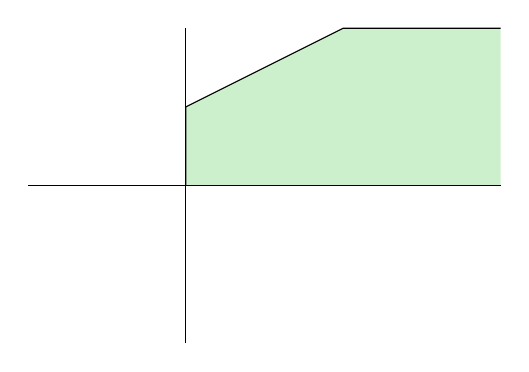
\begin{tikzpicture}

\fill[green!70!black!20!white] (0,0) -- (0,1) -- (2,2)  -- (4,2) -- (4,0) -- (0,0);
\draw (-2,0) -- (2,0);
\draw (0,-2) -- (0,2);
\draw (0,0) -- (0,1) -- (2,2)  -- (4,2);
\draw (0,0) -- (4,0);

\end{tikzpicture}
\end{figure}



\subsubsection{Soluciones factibles básicas}

Podemos dividir las columnas de $A$ es dos grupos $B$ y $N$, donde $B$ es $m\times m$ con $r(B)=m$.

\

\[
Ax=b \Leftrightarrow (B,N) {\comb{x_B}{x_N}}=b \Leftrightarrow B x_B + Nx_n = b
\]

\

Si hacemos $x_N=0$, $x_B=B^{-1}b$ y se verifica $B^{-1}b\geq 0$, obtenemos unos puntos especiales de $S$ que se llaman  \textbf{soluciones factibles básicas}.

\


Algunas soluciones del sistema compatible indeterminado $Ax=b$, con $r(A)=r(A,b)=m<n$ se consiguen fijando $n-m$ incógnitas como 0 y despejando las $m$ incógnitas restantes. Si estas soluciones son no negativas, son soluciones factibles básicas.

\obs Recordamos que en esta sección estamos tomando $S=\{x:\, Ax=b, x\geq 0\}$ \ref{subsec:AppOptLin}.

\begin{theorem}
$x$ es un punto extremo de $S$ $\dimplies$ $x$ es una solución factible básica.
\end{theorem}



\begin{proof}
Para la demostración, necesitamos enunciar un lema:
\begin{lemma}
Columnas de $A$ correspondientes a las coordenadas estrictamente positivas de un punto extremo son linealmente independientes.
\end{lemma}
\begin{proof}
Reordenamos la matriz $A$ para que las primeras sean linealmente independientes.


¿Porqué sabemos que son linealmente independientes? Si no lo fueran, entonces existen $λ_1,...,λ_k$ no todos nulos, tal que \[\sum_{i=1}^k λ_ia_k = 0 \]

Si definimos $λ \equiv (λ_1,...,λ_k,0,...,0)$, obtendríamos $\sum_i λ_ia_k = 0 \dimplies Aλ = 0$, lo cual es una contradicción con la independencia lineal.

\end{proof}


$\implies):$

Las columnas de la matriz $A$ correspondientes a las coordenadas positivas son linealmente independientes por el lema anterior. Tomamos un punto extremo $x$ y vamos a ver que tiene que ser solución factible.

Tomamos $\gor{x_1} = x + αλ$ y $\gor{x_2} = x-αλ$ son soluciones factibles. Para $α$ suficientemente pequeño, $\gor{x_1},\gor{x_2} > 0$

\[
A\gor{x_1} = A(x+αλ) = \underbrace{Ax}_{b} + α\underbrace{Aλ}_{0} = b
\]
\[
A\gor{x_2} = A(x-αλ) = \underbrace{Ax}_{b} - α\underbrace{Aλ}_{0} = b
\]

Entonces, $x$ no puede ser extremo, ya que es el punto medio de 2 puntos extremos.

$\impliedby):$ Se deja como ejercicio.

\end{proof}

Vamos a ver unos ejemplos para profundizar en el teorema:

\begin{example}
\[a_1x_1 + a_2x_2 + a_3x_3 = b\]
Con $x_i,b \geq 0$

Para sacar las soluciones factibles básicas, tomamos $a_1,a_2 = 0$ y despejamos $x_3$ para obtener una solución factible básica. Repitiendo el proceso tomando $a_2,a_3 = 0$ y $a_3,a_1 = 0$ obtenemos las 3 soluciones factibles básicas:

\[
\text{Soluciones } = \left( (\rfrac{a_1}{b},0,0), (0,\rfrac{a_2}{b},0) , (0,0,\rfrac{a_3}{b}) \right)
\]
En la \fref{fig:ejemploTriangulo} vemos gráficamente el problema que estamos tratando.

\begin{figure}[h!]
\centering
\begin{tikzpicture}
\draw[thick,->] (0,0,0) -- (4,0,0) node[anchor=north east]{$x$};
\draw[thick,->] (0,0,0) -- (0,3.5,0) node[anchor=north west]{$y$};
\draw[thick,->] (0,0,0) -- (0,0,3.5) node[anchor=west]{$z$};
\draw[fill=green!70!black!20!white,opacity=0.6] (2,0,0) -- (0,2,0) -- (0,0,2) -- cycle;
\node[nodepoint,label={above:$\rfrac{a_1}{b}$}] at (2,0,0) {};
\node[nodepoint,label={right:$\rfrac{a_2}{b}$}] at (0,2,0) {};
\node[nodepoint,label={left:$\rfrac{a_3}{b}$}] at (0,0,2) {};
\end{tikzpicture}
\caption{Ejemplo de coincidencia de soluciones factibles básicas con puntos extremos}
\label{fig:ejemploTriangulo}
\end{figure}

\end{example}

\begin{example}
\[a_1x_1 + a_2x_2 + a_3x_3 = b\]
Con $x_i,b \geq 0$ y además, $a_1 = a_2 = 0$.

Sólo tiene un vértice y sólo podemos calcular una solución factible básica. Ambas coinciden, con lo que el teorema se cumple.

\end{example}



La demostración implica que un punto extremo  no puede tener más de $m$ coordenadas estrictamente positivas. El recíproco no es cierto (veremos algún ejemplo más adelante en los ejercicios).

Si una solución factible básica tiene $k<m$ coordenadas estrictamente positivas se llama \concept{solución\IS factible básica degenerada}.

En el caso degenerado puede haber dos bases distintas $B$ y $B'$ que representen el mismo punto extremo. Esto se debe a que las $k$ columnas se pueden completar hasta las $m$ necesarias.


\begin{theorem}
El número de puntos extremos de $S$ es finito.

\end{theorem}

\begin{proof}
Elegir una base, que es elegir $n$ columnas de las $m$ posibles. Esto, como mucho se puede hacer como mucho de $\begin{pmatrix}n\\m\end{pmatrix}$ formas distintas.
\end{proof}



\begin{prop}
$S$ tiene al menos un punto extremo.
\end{prop}
\begin{proof}
Sea $x = (x_1,...,x_k,0,...,0)'$, con $x_i > 0,\; i=1,...,k$

Si las columnas correspondientes a las variables positivas ($a_1,...,a_k$) son linealmente independientes, completamos con las que nos hagan falta para formar una base.
Entonces $\{x_k\}$ es una solución factible básica, ya que:
\[Ax = (B,N)x = Bx_B = b \to x_B = B^{-1}b\geq 0 \to SFB\]
 Al ser $SFB$ tenemos que son puntos extremos.

 En caso de que las columnas correspondientes a las variables positivas ($a_1,...,a_k$) no sean linealmente independientes, vamos a ver qué ocurre utilizando un argumento similar al de la demostración del teorema de Caratheodory.

 \[(a_1,...,a_k) \to \exists λ_1,...,λ_k \tlq \sum a_iλ_i = 0\]

 Definimos \[\tilde{x} = \left\{\begin{array}{cc} x_i - αλ_i & i=1,..., k\\0& i=k+1,...,n\end{array}\right.\]

Buscamos que $\tilde{x}$ para que sea un punto extremo, es decir, que cumpla $A\tilde{x} = b$, con $\tilde{x} \geq 0$. Para ello, tenemos que \[A\tilde{x} = b = \sum_{i}^k(x_i - αλ_i)a_i = \sum x_ia_i \underset{=}{(1)} b\]

 $(1)$ se debe a que estamos en un conjunto factible.

Ahora sólo tenemos que definir $α$, e igualmente que en el teorema de Cara.., tomamos:
\[α = \min{\frac{x_i}{λ_i}, λ_i>0}\equiv \frac{x_r}{λ_r}\]

Y ahora repetiríamos el proceso, hasta quedarnos con un conjunto de $\{x_l\}$  tales que sus correspondientes columnas en $A$ sean linealmente independiente.
\end{proof}




\begin{example}
Vamos a estudiar el siguiente problema:

\begin{ioprob}
\goal{$\min -x_1 + 2x_2$}
\restrictions{$x_1+2x_2 \leq 2$}{$2x_1 + x_2\leq 1$}{$x_1\geq 0$}{$x_2\geq 0$}{}{}
\end{ioprob}

\begin{figure}[h]
\centering
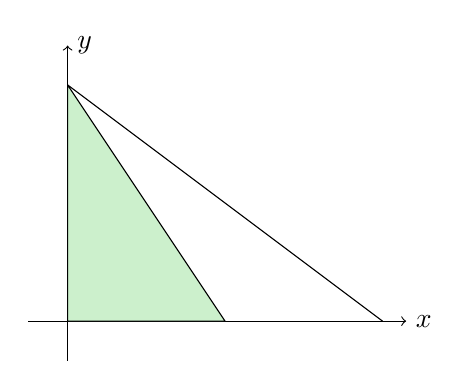
\begin{tikzpicture}
\draw[->] (-0.5,0) -- (4.3,0) node[right] {$x$};
\draw[->] (0,-0.5) -- (0,3.5) node[right] {$y$};;
\draw (4,0) -- (0,3);
\draw[fill=green!70!black!20!white] (0,0) -- (2,0) -- (0,3) -- cycle;
\end{tikzpicture}
\end{figure}

Añadimos las variables de holgura para pasarlo a forma normal estándar.

\begin{ioprob}
\goal{$\min -x_1 + 2x_2$}
\restrictions{$x_1+2x_2+x_3 \eq 2$}{$2x_1 + x_2 + x_4\eq 1$}{$x_1,x_2,x_3,x_4 \geq 0$}{}{}{}
\end{ioprob}

En este caso, tenemos:

\[A = \begin{pmatrix}1&2&1&0\\2&1&0&1\end{pmatrix}\;\; b = \begin{pmatrix}2\\1\end{pmatrix}\]

Operamos, tomando $B = \{a_1,a_2\}$: \[B = \begin{pmatrix}1&2\\2&1\end{pmatrix} \to B^{-1}b = \begin{pmatrix}\rfrac{-1}{3}&\rfrac{2}{3}\\\rfrac{2}{3}&\rfrac{-1}{3}\end{pmatrix}\begin{pmatrix}2\\1\end{pmatrix} = \begin{pmatrix}0\\1\end{pmatrix}\]

Hemos obtenido entonces:

\[x = \begin{pmatrix}X_b\\\hline X_n\end{pmatrix} = \begin{pmatrix}0\\1\\\hline0\\0\end{pmatrix}\]

Algo de soluciones degeneradas en este caso.

Vamos a ver que ocurre si tomamos las otras bases:

	\[B = \{a_1,a_3\} = \begin{pmatrix}1&1\\2&0\end{pmatrix} \to B^{-1}b = \begin{pmatrix}\rfrac{1}{2}\\\rfrac{3}{2}\end{pmatrix} \geq 0\]
	Entonces, tenemos $x = (\rfrac{1}{2},0,\rfrac{3}{2},0)$.

	Es importante en este caso, darse cuenta de que no son las primeras variables las principales y el resto las que son 0.

	\[B = \{a_1,a_4\} = \begin{pmatrix}1&0\\2&1\end{pmatrix} \to B^{-1}b = \begin{pmatrix}2\\-3\end{pmatrix} \not\geq 0\]
	En este caso, no tenemos una solución factible básica.

	 \[B = \{a_2,a_3\} = \begin{pmatrix}2&1\\1&0\end{pmatrix} \to B^{-1}b = \begin{pmatrix}1\\0\end{pmatrix} \not\geq 0\]
	 Teniendo $x = (0,1,0,0)$. En este caso, hemos obtenido la misma solución degenerada.


\obs La notación es realmente importante pillarla bien porque el algoritmo de Simplex la utiliza mucho.

$B$ = básicas. $N$ = No básicas.
\end{example}


\paragraph{Introducción al teorema:}

Tenemos $S = \{x : Ax = b, x\geq 0\}$. Queremos las direcciones tales que

\[A(x+λd) = b ∀λ>0 \dimplies Ad = 0\]
\[x+λd\geq 0 ∀λ>0 \dimplies d\geq 0\]


Tomamos $α>0$ en la coordenada $j$ de las coordenadas no básicas (coordenadas de $N$). Entonces, construimos:

\[d = \begin{pmatrix}-αB^{-1}a_j\\\hline 0\\\vdots\\ α\\ \vdots\\0\end{pmatrix} \]


\begin{theorem}[Caracterización\IS direcciones extremas]
Sea $d\in\real^n$ una dirección.

$d$ es una dirección extrema sí y sólo si $A = (B,N)$, donde $B$ es una matriz $m\times m$ básica, de manera que $B^{-1}a_j\leq 0$ para alguna de las columnas $a_j$ de $N$. Además,para algún $α>0$
\[d = \begin{pmatrix}-αB^{-1}a_j\\e_j\end{pmatrix}\]

donde $e_j = (\underbrace{0,...,0}_{j-1},1,0,...,0)$.
\end{theorem}

\begin{proof}
%% TODO:
Las demostraciones se dejan como ejercicio ya que son parecidas a la demostración del teorema de caracterización de puntos extremos.
\end{proof}

\begin{example}

\[S = \{(x_1,x_2)\in\mathbb{R}^2:\, x_2-x_1\leq 1,\, x_2\leq 2,\, x_1\geq 0,\, x_2\geq 0\}\]

Vamos a calcular sus direcciones extremas. Lo primero es escribirlo en forma estándar

\begin{ioprob}
\restrictions{$-x_1 + x_2 + x_3 = 1$}{$x_2+x_4 = 2$}{$x_i\geq 0$}{}{}{}
\end{ioprob}

La matriz $A$ es:

\[A = \begin{pmatrix}-1&1&1&0\\0&1&0&1\end{pmatrix}\; b = \begin{pmatrix}1\\2\end{pmatrix}\]

Vamos a dibujarlo para verlo:

\begin{figure}[h]
\centering
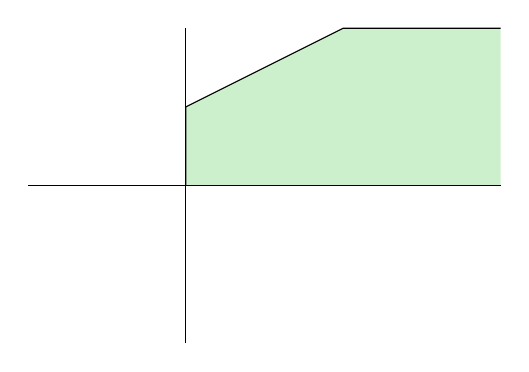
\begin{tikzpicture}
\fill[green!70!black!20!white] (0,0) -- (0,1) -- (2,2)  -- (4,2) -- (4,0) -- (0,0);
\draw (-2,0) -- (2,0);
\draw (0,-2) -- (0,2);
\draw (0,0) -- (0,1) -- (2,2)  -- (4,2);
\draw (0,0) -- (4,0);
\end{tikzpicture}
\end{figure}


Vamos a ver varios ejemplos de tomar varias bases:

\[
B = \{a_1,a_2\}, a_j = a_3 \to ... \to d = \begin{pmatrix}1\\0\\\hline1\\0\end{pmatrix}
\]
Encontramos la dirección extrema.

Podemos tomar otra columna no básica, y ver qué obtenemos:view
\[
B = \{a_1,a_2\}, a_j = a_4 \to ... \to d = \begin{pmatrix}\vdots\end{pmatrix}
\]

Esta base no ha sido elegida arbitrariamente. Aunque no tiene porqué ser la única base posible.
\end{example}

\begin{example}
Vamos a ver un ejemplo en $\real^3$. Tomamos $x_1 + x_2 = 1$, con $x_i \geq 0$.

Vamos a dibujarlo para verlo:

\begin{figure}[h]
\centering
\begin{tikzpicture}
\draw[thick,->] (0,0,0) -- (0,3.5,0) node[anchor=north west]{$z$};
\draw[thick,->] (0,0,0) -- (4,0,0) node[anchor=north east]{$y$};
\draw[thick,->] (0,0,0) -- (0,0,3.5) node[anchor=west]{$x$};
\draw[fill=green!70!black!20!white,opacity=0.6] (2,3,0) -- (2,0,0) -- (0,0,2) -- (0,3,2);
\node[nodepoint,label={above:$\rfrac{a_1}{b}$}] at (2,0,0) {};
\node[nodepoint,label={below:$\rfrac{a_2}{b}$}] at (0,0,2) {};
\end{tikzpicture}
\end{figure}
\end{example}

Seguimos caracterizando direcciones extremas.

\begin{prop}
El número de direcciones extremas es finito. En concreto,
\[\{\#\text{ direcciones extremas} \leq \comb{n}{m}(n-m)\]
\end{prop}

Vamos a ver un teorema, que de momento nos vamos a creer hasta que veamos el simplex.

\label{thm:representacion}
\begin{theorem}[Teorema\IS de representación]
 Sean $x_1,\ldots,x_k$ los puntos extremos de $S$ y sean $d_1,\ldots,d_\ell$ sus direcciones extremas. Entonces,
\[
x\in S \Leftrightarrow x = \sum_{i=1}^k \lambda_i x_i + \sum_{j=1}^\ell
 \mu_j d_j,
\]
donde $\lambda_i\geq 0$, $\mu_j\geq 0$, $\sum_{i=1}^k \lambda_i=1$.
\end{theorem}

En otras palabras, el conjunto se puede expresar como el cierre convexo de los vértices más una
combinación lineal positiva de las direcciones extremas.

\begin{figure}[h]
\centering
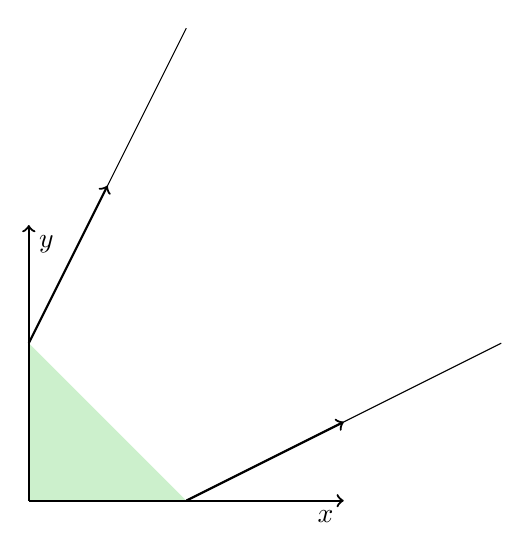
\begin{tikzpicture}
\fill[green!70!black!20!white] (0,0) -- (2,0) -- (0,2)  --  (0,0);
\draw[thick,->] (0,0) -- (0,3.5) node[anchor=north west]{$y$};
\draw[thick,->] (0,0) -- (4,0) node[anchor=north east]{$x$};
\draw[thick,->] (2,0) -- (4,1);
\draw[thick,->] (0,2) -- (1,4);
\draw[thin] (2,0) -- (6,2);
\draw[thin] (0,2) -- (2,6);
\end{tikzpicture}
\caption{Podemos "rellenar" el conjunto entero desplazando el cierre convexo a lo largo de las direcciones extremas}
\end{figure}







\section{Programación lineal}

Por el teorema de representación \ref{thm:representacion}, el problema lineal:


\begin{ioprob}
\goal{$\min c^\top x$}
\restrictions{$Ax=b$}{$x\geq 0$}{}{}{}{}
\end{ioprob}

es equivalente a:

\begin{ioprob}
\goal{$\min c^\top \left[\sum_{i=1}^k \lambda_i x_i + \sum_{j=1}^\ell \mu_j d_j\right]$}
\restrictions{$\sum_{i=1}^k \lambda_i=1$}{$\lambda_i\geq 0,\ i=1,\ldots,k$}{$\mu_j\geq 0,\ j=1,\ldots,\ell$}{}{}
\end{ioprob}

donde $x_1,\ldots, x_k$ son los puntos extremos del conjunto factible y  $d_1,\ldots,d_\ell$ son sus direcciones extremas.



\[\exists j c^td_j < 0 \to \text{ no existe solución}\]

Por la afirmación anterior, vamos a suponer que $c^td_i ∀i < l$. Entonces, es óptimo fijar $µ_i = 0∀i<l$. De esta manera, obtenemos el problema:
\begin{ioprob}
\goal{$\min c^\top \left[\sum_{i=1}^k \lambda_i x_i \right]$}
\restrictions{$\sum_{i=1}^k \lambda_i=1$}{$\lambda_i\geq 0,\ i=1,\ldots,k$}{$\mu_j\geq 0,\ j=1,\ldots,\ell$}{}{}
\end{ioprob}

Sea $j$ tal que $c^tx_j = \min{c^tx_i : i = 1,..., k}$. Entonces, es óptimo $λ_j = 1, λ_i = 0 ∀i≠j$.


\begin{figure}[h]
\centering
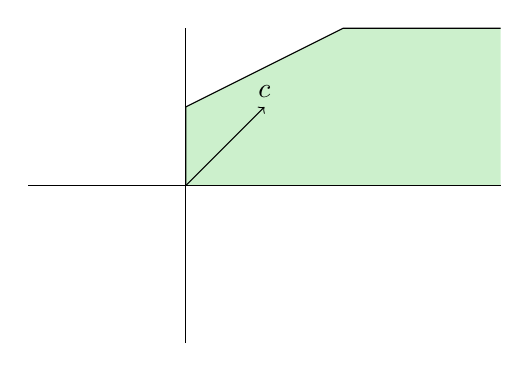
\begin{tikzpicture}
\fill[green!70!black!20!white] (0,0) -- (0,1) -- (2,2)  -- (4,2) -- (4,0) -- (0,0);
\draw (-2,0) -- (2,0);
\draw (0,-2) -- (0,2);
\draw (0,0) -- (0,1) -- (2,2)  -- (4,2);
\draw (0,0) -- (4,0);
\draw[->] (0,0) -- (1,1) node[above]{$c$};
\end{tikzpicture}
\end{figure}


¿Puede haber 2 soluciones factibles óptimas? En este caso, tendríamos $x_i$ y $x_j$ extremos tal que $c^tx_i = c^t = x_j = \min\{c^tx_i \}$. En este caso tenemos que $c^t(x_i - x_j) = 0 \to c\perp (x_i-x_j)$. En este caso, estamos en


\begin{figure}[h!]
\centering
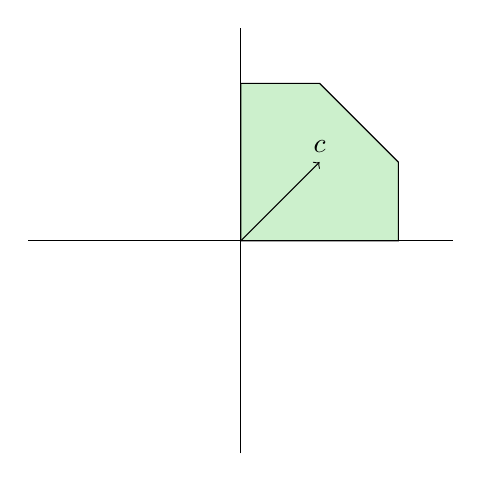
\begin{tikzpicture}
\fill[green!70!black!20!white] (0,0) -- (0,2) -- (1,2)  -- (2,1) -- (2,0) -- (0,0);
\draw (0,0) -- (0,2) -- (1,2)  -- (2,1) -- (2,0) -- (0,0);
\draw (-2.7,0) -- (2.7,0);
\draw (0,-2.7) -- (0,2.7);
\draw[->] (0,0) -- (1,1) node[above]{$c$};
\end{tikzpicture}
\caption{En este caso, existen muchas soluciones factibles óptimas Todas las del segmento.}
\end{figure}



\begin{theorem}[Teorema fundamental\IS de la programación lineal]


\end{theorem}

\subsection{Algoritmo del simplex.}


El algoritmo de simplex es un algoritmo de fuerza bruta.

Tenemos $B^{-1}b = \bar{b} \dimplies B\bar{b} = b$. Vemos que $\bar{b}$ es el vector $b$ en la base $B$.

El valor objetivo inicial es $\bar{z} = c^t\gor{x} = c^t_B\gor{x}_B = c^t_B\bar{b}$. Este es el valor objetivo que queremos mejorar. Vamos a tener que ponerlo todo en términos de la base $B$, entonces escribimos
-
\[Ax = b \dimplies Bx_B + Nx_N = b \dimplies x_B + B^{-1}Nx_N = \bar{b}\dimplies x_B = \bar{B} - B^{-1}NX_n \]
Hemos expresado las coordenadas básicas de cualquier punto factible en términos de la base $B$.

\obs \[Ax = b \dimplies Bx_B + Nx_N = b \] Es reescribirlo separando en parte básica ($B$) y parte no básica ($N$).


Finalizada la observación, vamos a ver el valor objetivo en cualquier punto factible $x=(x_B^\top,x_N^\top)^\top$:
\begin{align*}
z &= c_B^\top (\bar{b}-B^{-1} N x_N)+c^\top_N x_N =
 \bar{z}-(c_B^\top B^{-1} N - c_N^\top)x_N\\
  &=\bar{z}- \sum_{j\in N} (z_j-c_j)x_j,
\end{align*}
donde $z_j = c_B^\top B^{-1} a_j:= c_B^\top y_j$.

A las coordenadas de cada columna no básica en función de la base, lo llamamos $y_j$ (aunque debería llevar $\gor{y}$, no se la ponemos). Es decir
\[y_j=B^{-1} a_j\Leftrightarrow a_j = y_{1j} a_1+\cdots + y_{mj}a_m\]


\[
z = \bar{z}- \sum_{j\in N} (z_j-c_j)x_j.
\]


¿Qué ocurre si $z_j-c_j\leq 0$, para todo $j\in N$? Ocurre que entonces a $\bar{z}$ le sumamos algo, con lo que no mejoramos el valor objetivo, con lo que hemos llegado al óptimo.


En caso de no ser así, vamos a incluir en $B$ una variable de $N$. Llamaremos $x_k$ la variable no básica que incluimos como básica, y llamamos $x_r$ a la variable básica que dejar de ser básica ¿ya que $B$ se mantiene constante en dimensión?
Vamos a ver el criterio de entrada y de salida.

Sea $k \in N$ (no básico) tal que $z_k - c_k \ge 0$. En caso de haber varios $k$'s, tomamos el más alto, de tal manera que reduzcamos el valor objetivo lo más posible \footnote{Puede darse el caso de que en esta variable que reduce el valor objetivo no poodamos movernos casi porque estemos muy cerca del borde del conjunto}


El nuevo valor objetivo es: $\hat{z} =  \bar{z} - (z_k-c_k)\alpha$. Vamos a escribir el nuevo $\bar{b}$

\[A\hat{x} = b \dimplies  B\hat{x_B} + αNe_k \overset{\dimplies}{B^{-1}\times ...} \hat{x_B} + αy_k = \bar{b}\]
De esta manera, hemos llegado a $\hat{x_B} = \bar{b} - αy_k$ y $\hat{X_{N}} = αe_k$. Reescribiendo esta ecuación, podemos escribir:


\[\hat{x} = \bar{x} + \alpha\comb{-y_k}{e_k} \geq 0,\ \text{ donde }\ y_k=B^{-1}a_k\]

%\textcolor{red}{$\bar{b}$ se ha convertido en $\bar{x}$. No entiendo bien porqué es lo mismo.}

¿Qué ocurre con $y_k \leq 0$? Estamos en el caso que no tiene solución, ya que podemos aumentar $α$ todo lo que queramos.


Además, para que $\hat{x}$ sea factible también hace falta $\hat{x}\geq 0$:
\[
\hat{x}_B\geq 0\Leftrightarrow\bar{b}-\alpha y_k\geq 0\Leftrightarrow \alpha \leq \frac{\bar{b}_i}{y_{ik}},
\]
para todo $i=1,\ldots,m$ tal que $y_{ik}>0$.



\subsubsection{Ejemplos.}

\begin{example}

Vamos a aplicar el algoritmo de Simplex (aunque todavía no está formalmente muy definido) al problema:


\begin{ioprob}
\goal{$\max\{3x_1 + x_2 + 2x_3\}$}
\restrictions{$2x_1+x_2+x_3 \leq 2$}{$x_1 + 2x_2 + 3x_3\leq 5$}{$2x_1+2x_2+x_3\leq 6$}{$x_1\geq 0,\ x_2\geq 0,\ x_3\geq 0$}{}{}
\end{ioprob}


Pasamos primero a la forma estándar:

\begin{ioprob}
\goal{$\min\{-3x_1 - x_2 - 2x_3\}$}
\restrictions{$2x_1+x_2+x_3 + x_4 = 2$}{$x_1 + 2x_2 + 3x_3 +  x_5 = 5$}{$2x_1+2x_2+x_3 + x_6 = 6$}{$x_i\geq 0,\ i=1,\ldots,6.$}{}{}
\end{ioprob}


 
La solución factible básica inicial: $\bar{x}=(0,0,0,2,5,6)^\top$, para la que el objetivo es $\bar{z}=0$.

Tomamos:
\[B = \{a_4,a_5,a_6\} = I\]
\[\bar{b} = (2,5,6)^t \]
\[\bar{x} = (0,0,0,2,5,6) \]
\[c_B = (0,0,0)^t\]

\[
\begin{array}{cc}
y_1 = (2,1,2)' & z_1 - c_1 = c^t_By_1 - c_1 = 0 - (-3) = 3\\
y_2 = (1,2,2)' & z_2 - c_2 = c^t_By_2 - c_2 = 0 - (-1) = 1\\
y_3 = (1,3,2)' & z_3 - c_3 = c^t_By_3 - c_3 = 0 - (-2) = 2
\end{array}
\]

Ahora, incluimos $x_1$ ya que es la que más mejora el objetivo. Le corresponde $y_1$. ¿Cuánto podemos aumentar $x_1$? Pues sólo podemos aumentarlo:

\[ α = \min\{\rfrac{2}{2},\rfrac{5}{1},\rfrac{6}{2} \} = 1\]

Como el mínimo corresponde a la primera restricción, la variable que sale es la primera variable de la base, es decir $x_4$.

Ahora, en vez de invertir la matriz, vamos a utilizar el \textbf{pivote}\footnote{Ya lo veremos formalmente más adelante}, que consiste en obtener $(1,0,0)$ en la variable interesante, obteniendo:

\begin{align*}
2x_1+x_2+x_3 + x_4 &= 2   \\
x_1 + 2x_2 + 3x_3 +  x_5 &= 5  \\
2x_1+2x_2+x_3 + x_6 &= 6 
\end{align*}

Vamos a calcular:
\[
\begin{array}{cc}
y_? =  & z_2 - c_2 = c^t_By_2 - c_2 = (-3,0,0)\begin{pmatrix}\rfrac{1}{2}\\\rfrac{3}{2}\\\rfrac{5}{2}\end{pmatrix} - (-1) = -\rfrac{1}{2}\\
y_2 = (1,2,2)' & z_3- c_3 = c^t_By_3 - c_3 = (-3,0,0)\begin{pmatrix}\rfrac{1}{5}\\\rfrac{5}{2}\\0 \end{pmatrix} - (-2) = \rfrac{1}{2}\\
y_3 = (1,3,2)' & z_4 - c_4 = c^t_By_4 - c_4 = .. = -\rfrac{3}{2}
\end{array}
\]

La mayor (y además, la única positiva) es $x_3$. Esta es la variable que entra en la base.

Como $y_3 > 0$, vamos a tener solución. Si $y_3 < 0$, podríamos aumentar todo lo que quisiéramos $x_3$ mejorando siempre el objetivo. Ahora, calculamos $α$

\[α = \min\left\{\frac{1}{\rfrac{1}{2}}, \frac{4}{\rfrac{5}{2}}\right\} = \frac{8}{5}\]

La variable que sale es la que tiene de coeficiente de $x_3 = \rfrac{8}{5}$, es decir, $x_5$.

Ya hemos hecho 2 iteraciones del algoritmo y son suficientes. Pero ahora, nos surge la duda, ¿vamos a acabar en algún momento?
Si todos los $\bar{b}$ son positivos, entonces siempre tendremos solución. Si en algún caso tenemos $\bar{b}_r = 0 \implies α=0$. Esto provoca que tengamos bases distintas que den lugar a la misma solución.
Esto se da cuando hay degeneración. ¿Cómo solucionarlo? Pues otra posibilidad es cambiar el criterio de entrada y salida de variable. La \concept{regla\IS de Bland} consiste en escoger la variable de menor índice. 
No vamos a ver la demostración porque es muy engorrosa, pero esta regla nos da una solución óptima incluso con el caso degenerado.
\end{example}


  
\subsubsection{La tabla del simplex. Pivoteo.}

Una vez visto el algoritmo entendiéndolo, vamos a ver cómo hacer las cuentas de una manera más ordenada y optimizada. Para ello, vamos a construir la \concept{tabla\IS simplex}


\begin{table}
\centering
\begin{tabular}{c||c|c}
$c$ & $c_B^\top$  & $c^\top_N$ \\ \hline\hline
Variables & $x_B^\top$ &  $x^\top_N$ \\ \hline
$x_B=\bar{b}$ &    $\mathbb{I}_{m\times m}$ & $B^{-1}N$ \\ \hline
$z-c$   & $0$   & $c_B^\top B^{-1}N - c^\top_N$
\end{tabular}
\label{tbl:simplex}
\caption{Tabla simplex en la que resumir cada iteración.}
\end{table}


\begin{example}

Vamos a ver un laaaargo ejemplo de cómo se aplica el algoritmo para este problema:

\begin{ioprob}
\goal{$\min\{-4x_1 - 3x_2\}$}
\restrictions{$-x_1+x_2+x_3  = 2$}{$x_1 + 2x_2 + x_4 = 6$}{$2x_1+x_2 + x_5 = 6$}{$x_i\geq 0,\ i=1,\ldots,5.$}{}{}
\end{ioprob}


\textbf{Tabla inicial:}  $B=(a_3,a_4,a_5) = \mathbb{I}_{3\times 3}$



\begin{table}
\centering
\begin{tabular}{r | rrrrr}
$c$ & -4 & -3 & 0 & 0 & 0 \\ \hline
Variables & $x_1$ & $x_2$ & $x_3$ & $x_4$ & $x_5$ \\ \hline
$x_3 = 2$ & -1 & 1 & 1 & 0 & 0 \\
$x_4=6$   & 1 & 2 & 0 & 1 & 0  \\
$x_5=6$ & 2 & 1 & 0 & 0 & 1 \\ \hline
$z_j-c_j$ & 4 & 3 & 0 & 0 & 0 
\end{tabular}
\end{table}

Como en la última fila hay valores positivos, tenemos que seguir iterando. 

La variable que sale es $x_5$ y la que entra es la $x_1$, ya que $\rfrac{6}{2}$ es el menor de los cocientes de:

\[\min\left\{\frac{\gor{b}_j}{y_{jk}}: y_{jk}>0\right\}\]

\paragraph{Reemplazo:}

Ahora vamos a reemplazar. Para ello, necesitamos conseguir en la primera columna el $(0,0,1)'$ para sustituir al $(-1,1,2)$ (esto es pivotear).

\begin{table}
\centering
\begin{tabular}{r | rrrrr}
$c$ & -4 & -3 & 0 & 0 & 0 \\ \hline
Variables & $x_1$ & $x_2$ & $x_3$ & $x_4$ & $x_5$ \\ \hline
$x_3=5$ & 0 & 3/2 & 1 & 0 & 1/2 \\
$x_4=3$   & 0 & 3/2 & 0 & 1 & -1/2  \\
$x_1=3$ & 1 & 1/2 & 0 & 0 & 1/2 \\ \hline
$z_j-c_j$ &  0 & 1 & 0 & 0 & -2 
\end{tabular}
\end{table}

Como vemos que sigue habiendo un valor positivo, podemos obtener un valor mejor, iteramos otra vez, obteniendo:

\begin{table}
\centering
\begin{tabular}{r | rrrrr}
$c$ & -4 & -3 & 0 & 0 & 0 \\ \hline
Variables & $x_1$ & $x_2$ & $x_3$ & $x_4$ & $x_5$ \\ \hline
$x_3=2$ & 0 & 0 & 1 & -1 & 1 \\
$x_2=2$   & 0 & 1 & 0 & 2/3 & -1/3  \\
$x_1=2$ & 1 & 0 & 0 & -1/3 & 2/3 \\ \hline
$z_j-c_j$ &  0 & 0 & 0 & -2/3 & -5/3 
\end{tabular}
\end{table}

Ahora ya hemos terminado, porque la última fila ya no tiene valores positivo. Ahora, para construir la solución, escribimos:

\[SFO = (x_3,x_2,x_1,0,0)' = (2,2,2,0,0)'\]

\end{example}

\subsubsection{Método de las dos fases.}

\subsection{Optimización lineal con {\tt R}}

